\section{FermiChopper: The Fermi-chopper}

\component{FermiChopper}{M. Poehlmann, C. Carbogno, H. Schober, E. Farhi}{$R,y_{min} y_{max}, \nu,w,length$,Nslit,phase}{$m,Q_c,R_0,\alpha, W$,curvature,zero\_time}{validated}
\index{Optics!Fermi Chopper|textbf}

\begin{figure}
\begin{center}
\begin{tabular}{cc}
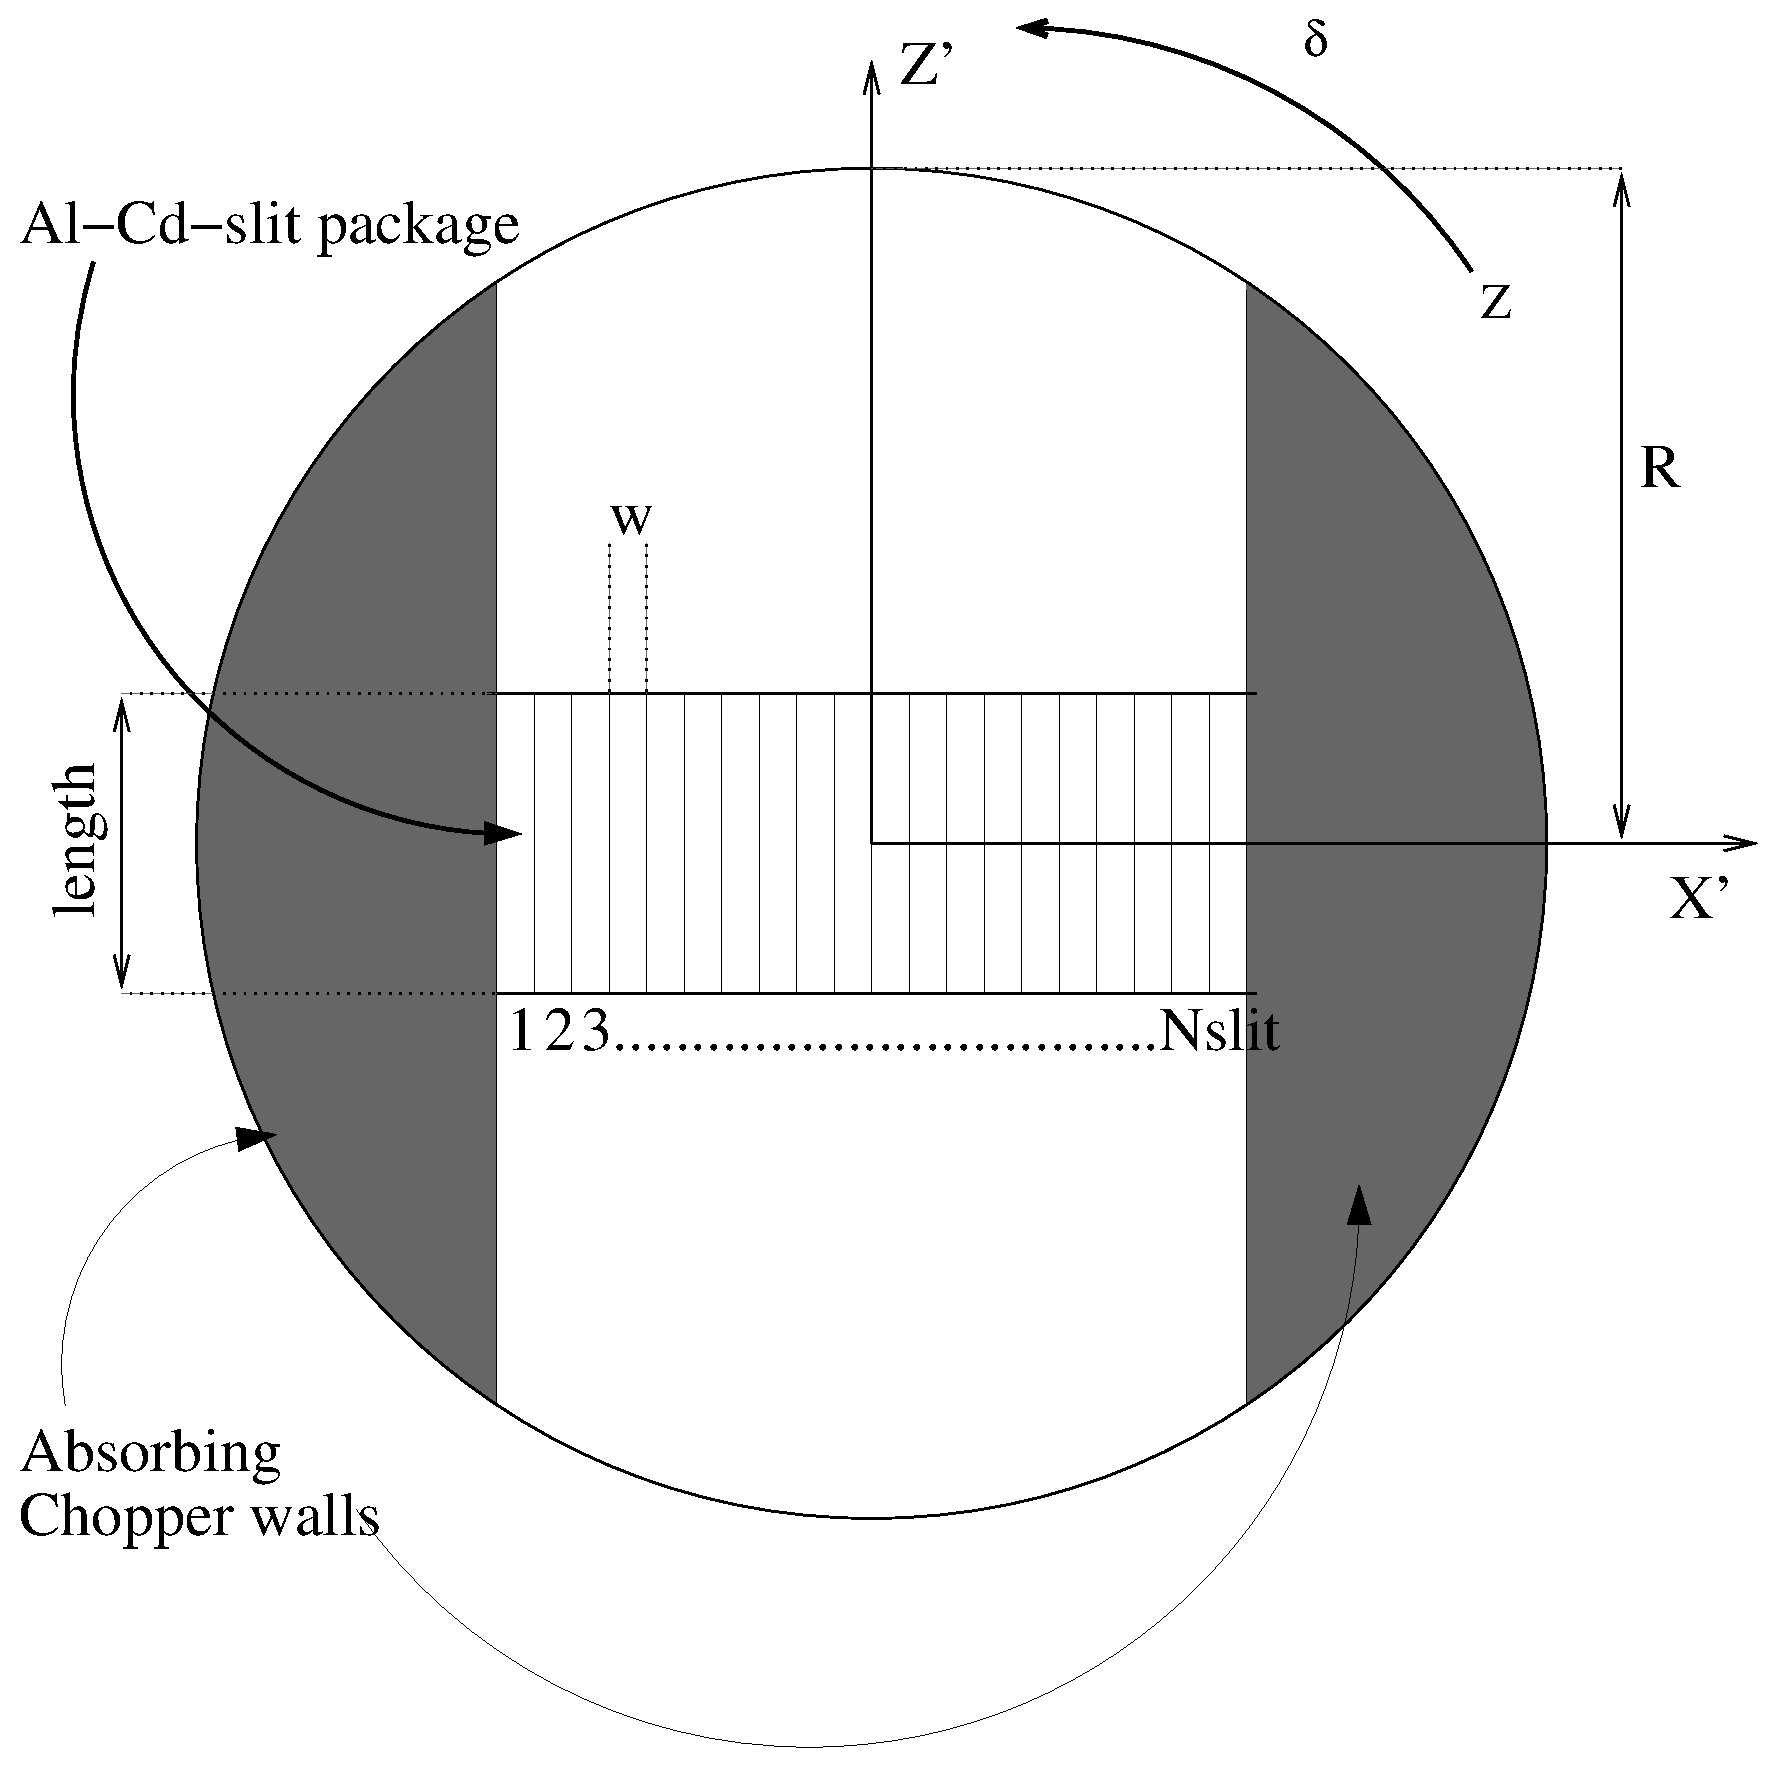
\includegraphics[height=7cm]{./figures/FCChoppergeo.eps}
&
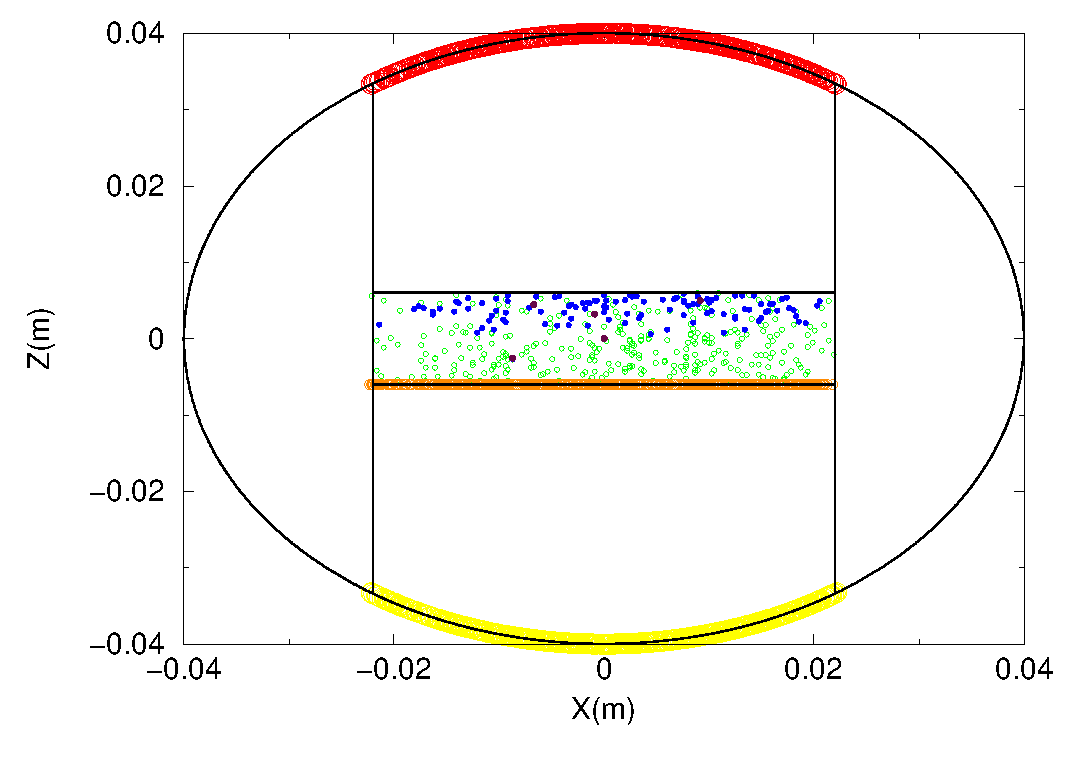
\includegraphics[height=5cm,width=5.3cm]{./figures/FCOverview.eps}
\end{tabular}
\end{center}
\caption{Geometry of the Fermi-chopper (left) and Neutrons in the chopper (right).}
\label{fig:Overview.eps}
\end{figure}

\subsection{The chopper geometry and parameters}
\label{ssec:chopper}

The Fermi chopper is a rotating vertical cylinder containing a set of collimating slits (\emph{slit package}). Main geometry parameters are the radius $R$, minimum and maximum height $y_{min}$ and $y_{max}$ (see Fig. \ref{fig:Overview.eps}).
In this implementation, the slits are by default straight, but may be coated with super-mirror, and curved. Main parameters for the slits are the number of slits $Nslit$, the length $length$ and width $w$ of each slit, the width of the separating Cd-blades is neglected. The slit walls reflectivity is modelled just like in guide components by the $m$-value ($m > 1$ for super mirrors), the critical scattering vector $Q_c$, the slope of reflectivity $\alpha$, the low-angle reflectivity $R_0$ and the width of supermirror cut-off $W$. For $m=0$ the blades are completly absorbing. The AT position of the component is its center.

The angular speed of the chopper is $\omega = 2\pi \nu$, where $\nu$ is the rotation frequency. The angle $phase$ for which the chopper is in the 'open' state for most of the neutrons coming in (z' axis of the rotating frame parallel to the z axis of the static frame) is also an input parameter. The time window may optionally be shifted to zero when setting the \verb+zero_time=1+ option. A phase guess vaue may be set automatically using the \verb+zero_time=2+ option.

The curvature of the slit channels is specified with the {\it curvature} parameter. Positive sign indicates that the deviation 'bump' due to curvature is in the $x'$ positive side, and the center of curvature is in the $x'$ negative side. The optimal radius of curvature $R$ is related to frequency $\nu$ and neutron velocity $v$ with: $v=4 \pi R \nu$.

The component was validated extensivelly by K. Lieutenant. As an alternative, one may use the {\bf Vitess\_ChopperFermi} component (eventhough slower and without super-mirror support) or the {\bf FermiChopper\_ILL} contributed component. The Guide\_gravity componnt has also a rotating mode, using an approximation of a Fermi Chopper.

\begin{table}
  \begin{center}
  {\let\my=\\
    \begin{tabular}{|lr|p{0.6\textwidth}|}
    \hline
Parameter & unit & meaning \\
    \hline
radius & [m] & chopper cylinder radius \\
ymin   & [m] &   lower y bound of cylinder \\
ymax   & [m] &   upper y bound of cylinder \\
Nslit  & [1] &   number of chopper slits \\
length & [m] &   channel length of the Fermi chopper \\
w      & [m] &   width of one chopper slit. May also be specified as \emph{width}=w*Nslit for total width of slit package. \\
nu & [Hz] &  chopper frequency \\
phase     & [deg] &   chopper phase at t=0 \\
zero\_time & [1] & shit time window around 0 if true \\
curvature & [m$^{-1}$] & Curvature of slits (1/radius of curvature) \\
    \hline
m     & [1] & \\
alpha & [\AA] & \\
Qc    & [\AA$^{-1}$] & slit coating parameters. See section \ref{ss:mirrorreflect} \\
W     & [\AA$^{-1}$] & \\
R0    & [1] & \\
    \hline
    \end{tabular}
    \caption{FermiChopper component parameters}
    \label{t:fc-param}
  }
  \end{center}
\end{table}


\subsection{Propagation in the Fermi-chopper}

As can be seen in figure \ref{fig:Overview.eps}, neutrons first propagate onto the cylinder surface of the chopper (yellow curve). Then the program checks the interaction with the entrance of the slit package (orange line) and calculates which slit is hit. If the slit coating is reflecting ($m > 0$), multiple reflections are calculated (green, blue and maroon circles), otherwise the neutrons are absorbed as soon as they interact with the blades. Finally the remaining neutrons propagate to the exit of the chopper (red curve).

The rotation of the chopper is characterized by the angle $\delta$ between the rotating z' and the static z-axis. $\delta(t)$ is defined by:

$$\delta(t) = \widehat{z,z'} = \omega.(t-t_0)$$

where $t$ is the absolute time. The chopper should better be \emph{time focussing}: slow neutrons should pass before the fast ones, so that they finally hit the detectors at the same time. Therefore the signs of $\omega$ and $\delta$ are very important: For $t>t_0$, $\delta$ is positive and points anti-clockwise.

Since the rotation is applied along the y - axis, we can simplify the problem to two dimensions. The orthogonal transformation matrix $T$ from the static $(xz)$ to the rotating frame $(x'z')$ is:
\begin{equation}
T_{xz \rightarrow x'z'} = \left(
\begin{array}{cc}
\cos(\delta) & \sin (\delta) \\
-\sin(\delta) & \cos(\delta)
\end{array}
\right)
\end{equation}

\begin{figure}
\begin{center}
\begin{tabular}{cc}
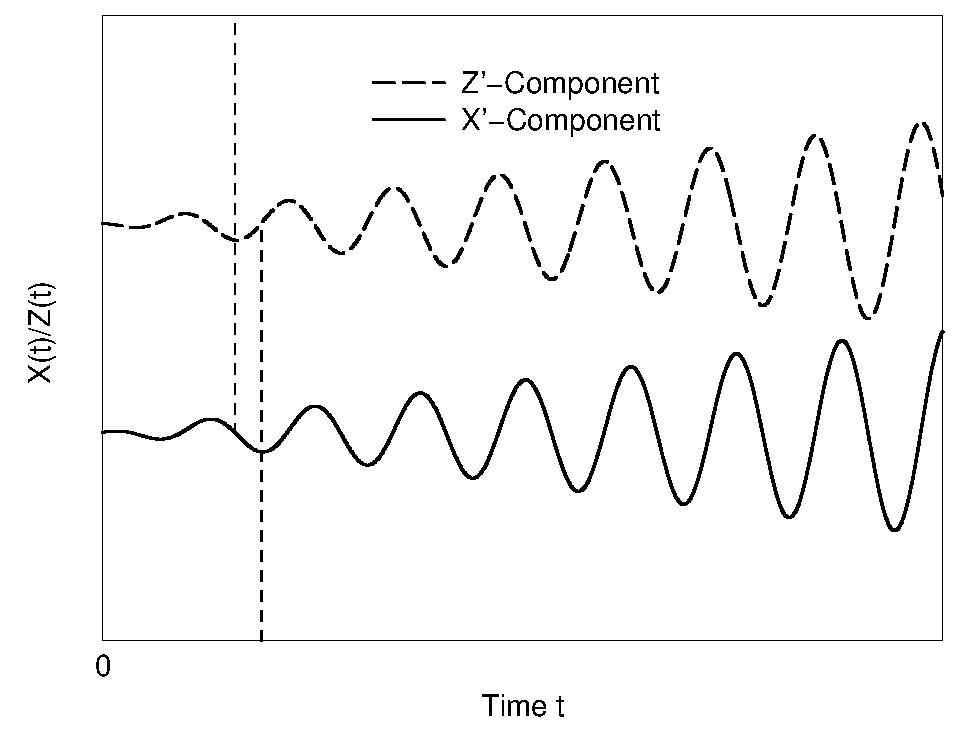
\includegraphics[height=5.5cm]{./figures/XZCoords.eps}
&
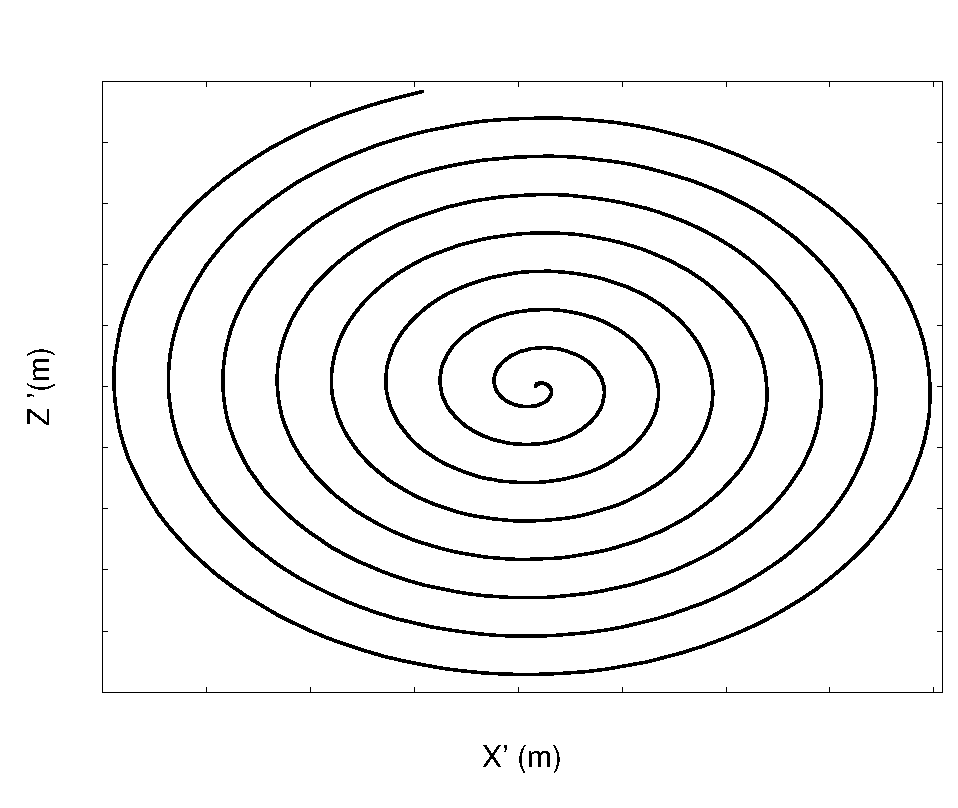
\includegraphics[height=6.5cm,width=5.5cm]{./figures/XZplain.eps}
\end{tabular}
\end{center}
\caption{The x' and z' component as a function of time in the rotating frame (left). A typical neutron trajectory in the rotating frame (right).}
\label{fig:Component.eps}
\end{figure}

Together with the equation for a non-accelerated, linear propagation $\vec{r} = \vec{r_0}+\vec{v}t$ the orthogonal transformation produces a curve in the X'-Z'-plane known as \emph{archidemic spiral}, as can be seen in figure \ref{fig:Component.eps}. The two vector components $s(t) = (x',z')$ follow the equation:
\begin{equation}
s(t) = \left(
\begin{array}{c}
x' \\
z'
\end{array}
\right) = T.\left(
\begin{array}{c}
x(t) \\
z(t)
\end{array}
\right) = \left(
\begin{array}{c}
(x_0+v_x.t)cos(\delta(t)) + (z_0+v_z.t)sin(\delta(t)) \\
-(x_0+v_x.t)sin(\delta(t)) + (z_0+v_z.t)cos(\delta(t))
\end{array}
\right).
\label{eq:Txz}
\end{equation}
For a fixed chopper rotation speed, the neutron trajectory tends to strech from a spiral curve for slow neutrons to a straight line for fast neutrons. For real Fermi chopper settings $\nu$ (about 100 Hz on IN6 at the ILL), neutron trajectories are found to be nearly straight for 1000 m/s neutron velocities \cite{blanc83}.

The basis of the algorithm is to find the intersections of these spiral trajectories with the chopper outer cylinder and then the slit package, in the rotating frame.

For this purpose, the \emph{Ridders's} root finding method was implemented \cite{NumRecip} in order to solve
\begin{equation}
x'(t) = d {\rm\ or\ } z'(t) = d
\label{eq:Ridder}
\end{equation}
This method provides faster and more accurate intersection determination than other common algorithms. E.g. the secant method fails more often and may give wrong results (outside chopper) whereas the bisection method (a.k.a Picard dichotomy) is slightly slower.

\subsubsection{Standard slit packages (non super-mirror)}

\begin{figure}
\begin{center}
\begin{tabular}{cc}
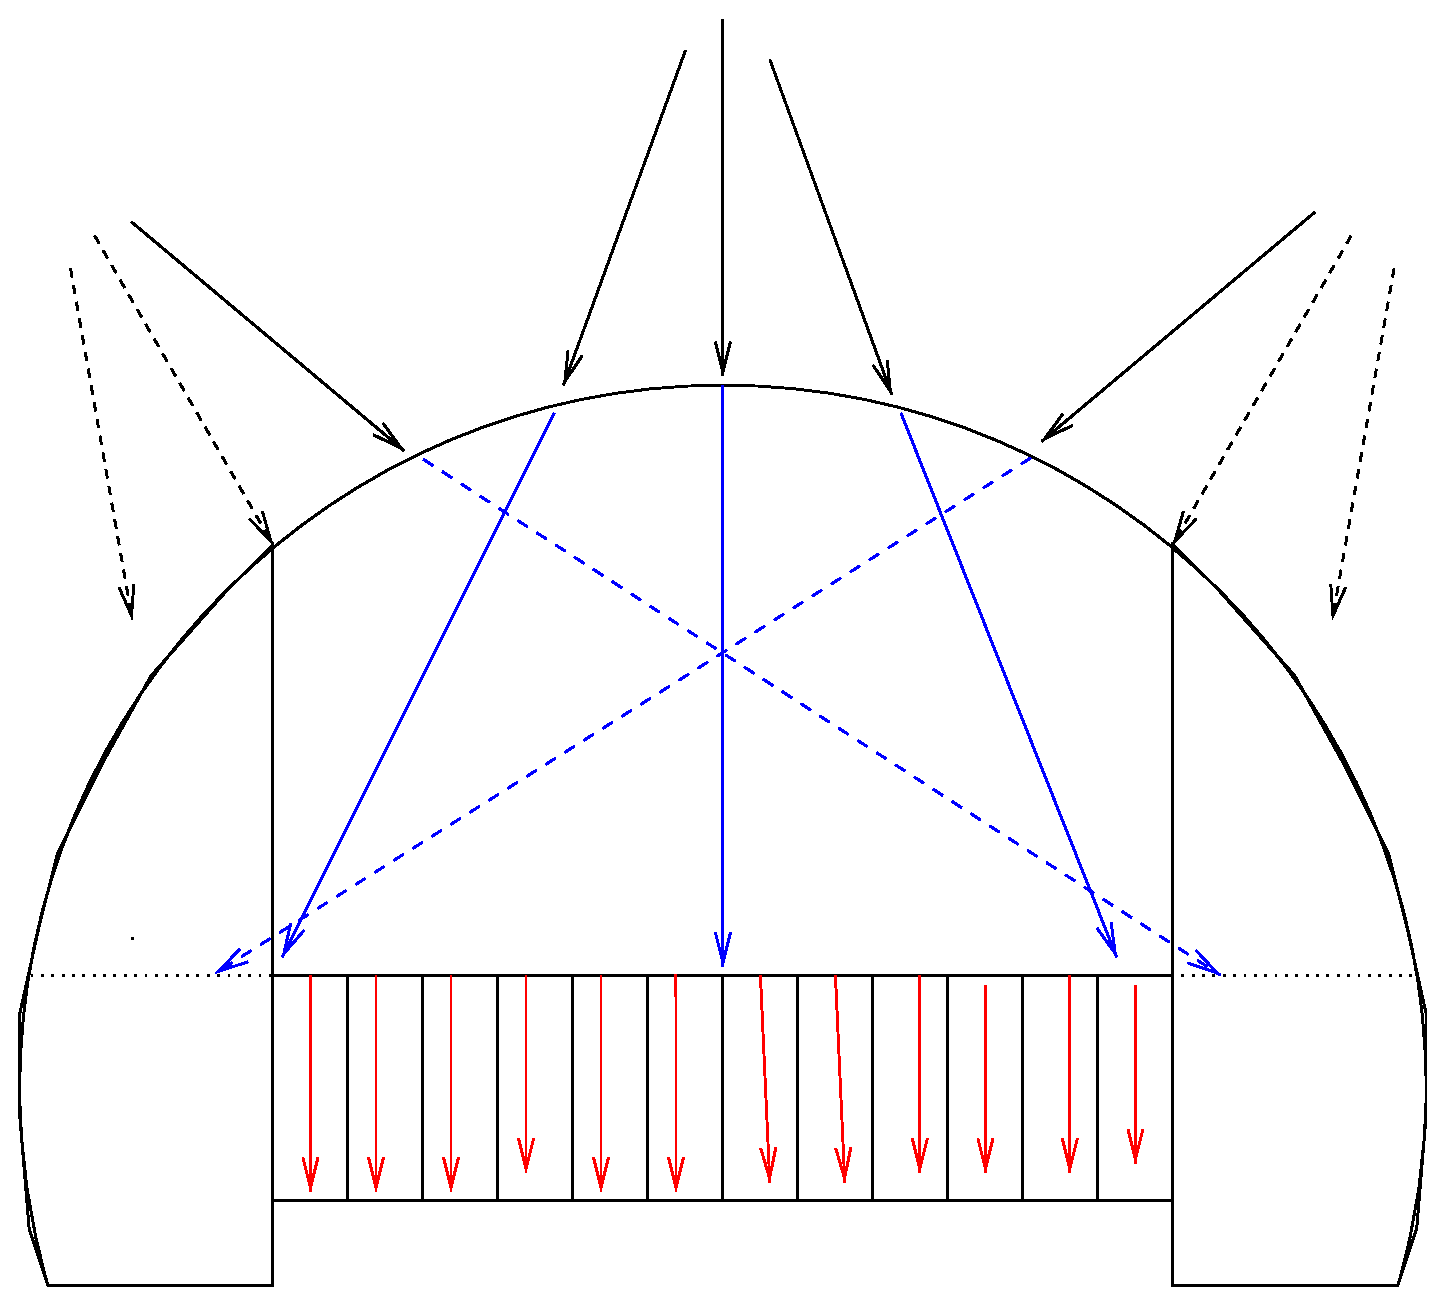
\includegraphics[height=5cm]{./figures/FCAlgo.eps}
&
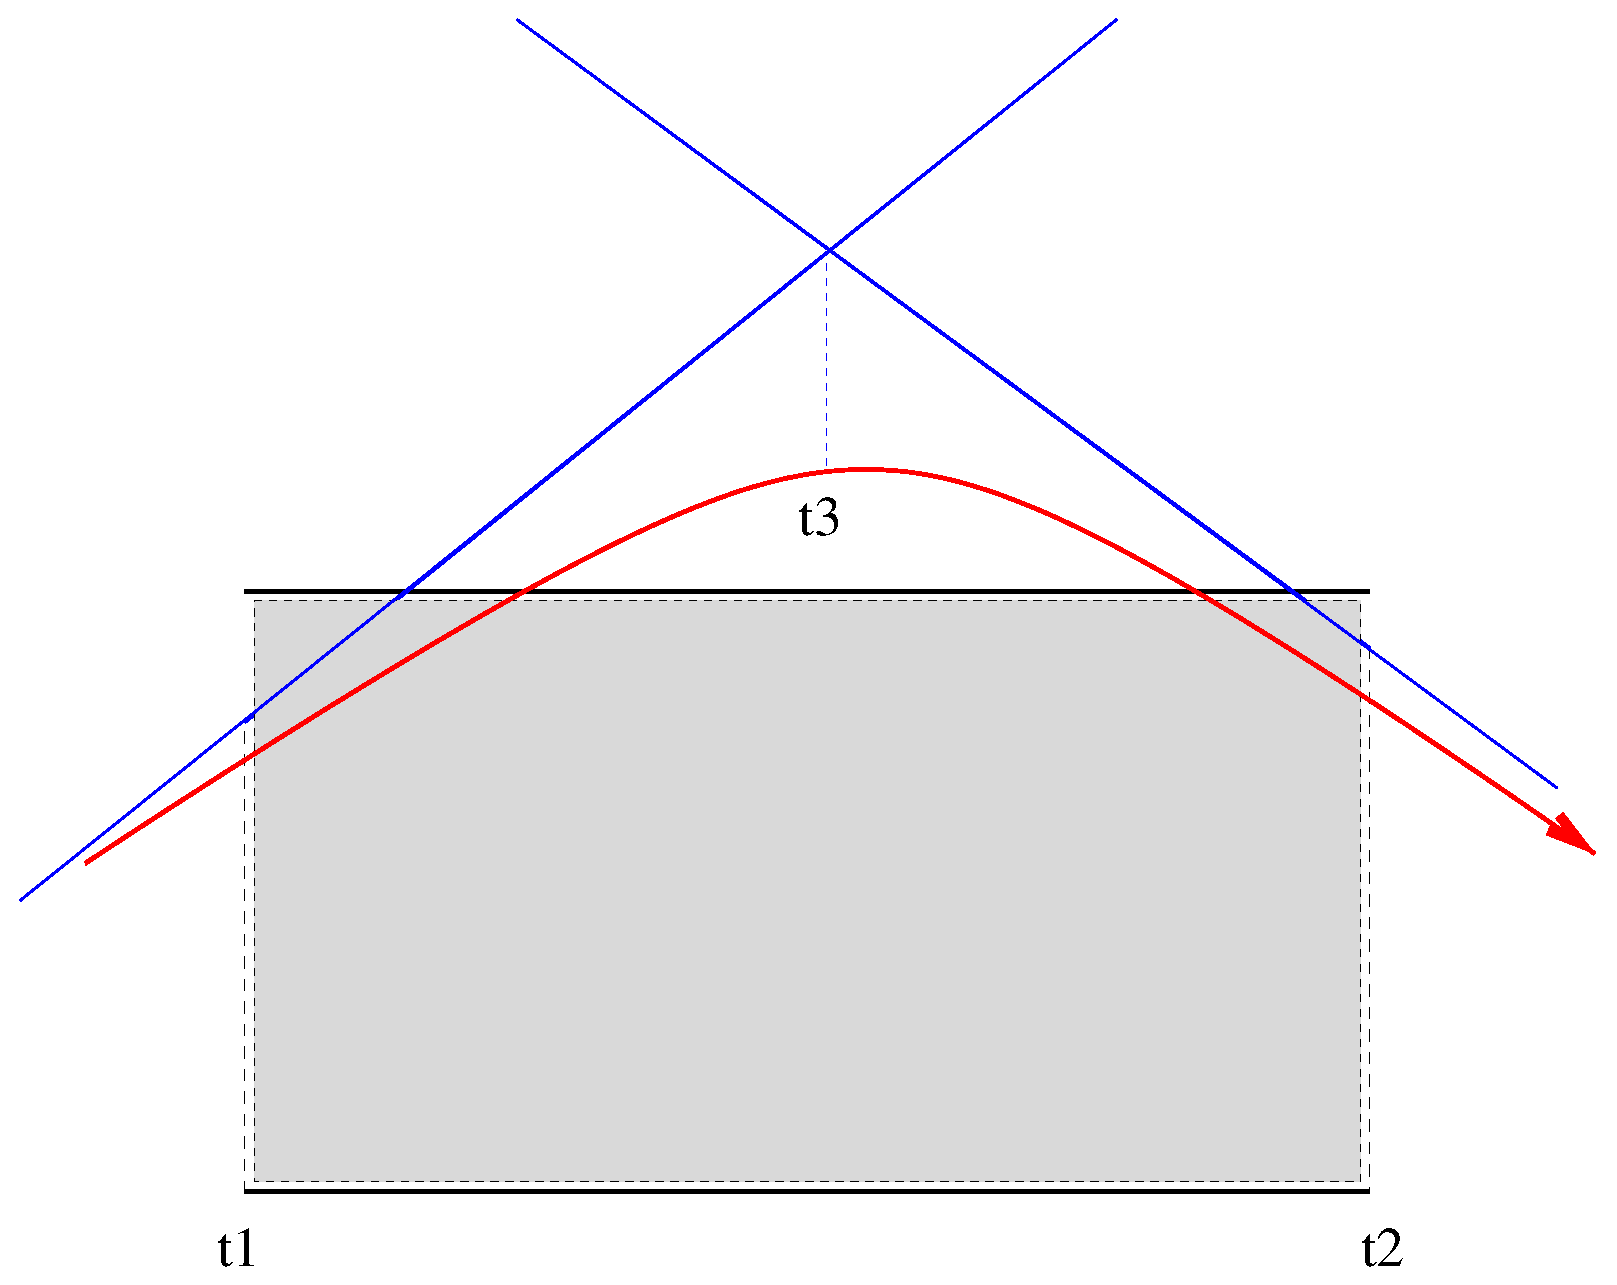
\includegraphics[height=5cm]{./figures/FCtangents.eps}
\end{tabular}
\end{center}
\caption{The different steps in the algorithm (left). A neutron trajectory in a slit (right)}
\label{fig:TOFalg.eps}
\end{figure}

The neutrons are first propagated to the outer chopper cylinder and their coordinates are transformed into the rotating frame using $T$. Neutrons outside the slit channel (chopper opening), or hitting the top and bottom caps are absorbed (yellow dots in Fig. \ref{fig:Overview.eps}). The side from which the neutron approaches the chopper is known (positive or negative z'-axis of the rotating frame) so that the calculation of the time of interaction with the slit package entrance $t_1$ is performed solving $z' = \pm \frac{\rm length}{2}$ in Eq. (\ref{eq:Txz}). Using the result of the numerical algorithms the neutron propagates to the entrance of the slit package (orange circles in Fig. \ref{fig:Overview.eps}). Neutrons getting aside the slit package entrance are absorbed. Additionally, the slit package exit time $t_2$ is estimated the same way with $z' = \mp \frac{\rm length}{2}$, in order to evaluate the whole time-of-flight in the chopper. The index of the slit which was hit is also computed, as we know the $x'$ coordinate in the rotating frame at the slit entrance.

Differentiating Eq. (\ref{eq:Txz}) for $x$ coordinate
\begin{equation}
\dot{x'}(t) = v_x'(t) = [v_x+\omega.(z+v_z(t))]\cos(\omega(t-t_0))
+ [v_z-\omega.(x+v_x(t))]\sin(\omega(t-t_0))
\end{equation}
we may estimate the tangents to the spiral neutron trajectory in the rotating frame at times $t_1$ and $t_2$. The intersection of these two lines gives an intermediate time $t_3$.

If the neutron remains in the same slit at this point, then there is no intersection with the slit walls (direct flight), and the neutron may be propagated to the slit output, and then to the cylinder output. A last check is made for the neutron to pass the chopper aperture in the cylinder.

If the neutron changes of slit channel at this point, we may determine the intersection time of the neutron trajectory within $[ t_1, t_3 ]$ or $[ t_3, t_2 ]$, as seen in Fig. \ref{fig:TOFalg.eps}. If walls are not reflecting, we just absorb neutrons here.

\subsubsection{The reflections (super-mirror slits)}

If slit walls are reflecting, neutron is first propagated to the slit separating surface. Then the velocity in the rotating frame is computed using Eq. (\ref{eq:Txz}). Perpendicular velocity $v_x'$ is reverted for reflection, and inverse $T$ transformation is performed. Reflected intensity is computed the same way as for the guide component (see section \ref{s:mirror}). The remaining time $t_2$ to the slit output is estimated and the tangent intersection process is iterated, until neutron exits. Remember that super mirror $m < 1$ parameters behave like $m=1$ materials (see section \ref{ss:mirrorreflect}).

The propagation is finalized when determining the intersection of the neutron trajectory with the outer surface of the chopper cylinder. The neutron must then pass its aperture, else it is absorbed.

\subsubsection{Curved slit packages}

The effect of curvature can significantly improve the flux and energy resolution shape.

As all $(xz)$ cordinates are transformed into $(x'z')$, the most efficient way to take into account the curvature is to include it in the transformation Eq. (\ref{eq:Txz}) by 'morphing' the curved rotating real space to a straight still frame. We use parabolic curvature for slits. Then instead of solving
\begin{equation}x'(t) = d - \Delta_{x'}(z') {\rm\ where\ } \Delta_{x'}(z')=R_{slit}.(1-\sqrt{1-(z'/R_{slit})^2})
\end{equation}
with $\Delta$ being the gap between the straight tangent line at the slit center and the real slit shape, we perform the additional transformation
\begin{equation}
x' \rightarrow x' + \Delta_{x'}(z')
\end{equation}
The additional transformation counter-balance the real curvature so that the rest of the algorithm is written as if slits were straight.
This applies to all computations in the rotating frame, and thus as well to reflections on super mirror coatings.
